\documentclass{article}
\usepackage{graphicx}
\usepackage[margin=1.5cm]{geometry}
\usepackage{amsmath}

\begin{document}

\title{Thursday Reading Assessment: Chapters 4-5}
\author{Prof. Jordan C. Hanson}

\maketitle

\begin{figure}[ht]
\centering
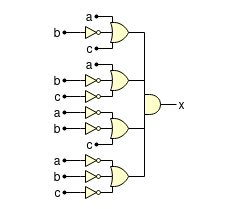
\includegraphics[width=0.33\textwidth]{figures/SPOS_example.png}
\caption{\label{fig:1} A logic function in need of simplification.}
\end{figure}

\section{Logic Circuits, Boolean Algebra, and Karnaugh Maps}

\begin{enumerate}
\item Consider the logic function in Fig. \ref{fig:1}.  (a) Based on Fig. \ref{fig:1}, write an S-POS expression for the output. (b) From the S-POS expression, create the Karnaugh map and the truth table. (c) Generate the simplified Boolean expression from the Karnaugh map.  \textit{Hint: remember that cells in the top row are adjacent to those in the bottom row.} \\ \vspace{4cm}
\item Draw the simplified logic function diagram using basic gates.
\end{enumerate}

\end{document}
